\documentclass[
    12pt,
    a4paper,
    ngerman,
    color=3b,% Farbe für Hervorhebungen auf Basis der Deklarationen in den
    %type=intern,
    %titlepage=true,
    marginpar=false,
    colorback=false,
    %logo=head,
    leqno,
]{tudaexercise}
\usepackage{import}
% Import all Packages from Main Preamble with relative Path
\subimport*{../../}{preamble}
% Get Labels from Main Document using the xr-hyper Package
\externaldocument{../../AuD-Zusammenfassung-2020}
% Set Graphics Path, so pictures load correctly
\graphicspath{{../../}}

\begin{document}
\section{NP}\index{NP}
\begin{itemize}
    \item \fatsf{Berechnungsprobleme}\\
    
\includegraphics[width=.5\textwidth]{pictures/npmeme.png}
          \begin{itemize}
              \item Sind alle Probleme in polynomieller Zeit lösbar? ($O(n^k)$)
              \item Nein $\Rightarrow$ Manche nur in superpolynomieller Zeit lösbar
              \item Polynomielle Probleme: \textit{\string"einfach\string"}
              \item Superpolynomielle Probleme: \textit{\string"hart\string"}
          \end{itemize}

    \item \fatsf{Klasse P}
          \begin{itemize}
              \item Klasse aller Polynomialzeitprobleme
              \item Problem ist \textit{effizient lösbar} gdw. es in polynomieller Zeit lösbar ist
              \item Gilt für Polynome beliebigen Grades (auch $n^k$)
              \item Zeitkomplexität $n^k$ mit gro\ss em $k$ bedenklich, jedoch fast nie notwendig
              \item $n$ beschreibt die Länge der Eingabe
              \item Beispiele: Binäre Addition, Kürzeste Wege, Sortieren,...
          \end{itemize}

    \item \fatsf{Klasse NP}
          \begin{itemize}
              \item Enthält \textit{\string"einfach zu verifizierende\string"} Probleme (polynomieller Zeit)
              \item Enthält Probleme mit \textit{\string"kurzem Beweis\string"} (Länge polynomiell in Länge der Instanz)
              \item Also: Klasse aller Probleme, deren Lösung in Polynomialzeit verifizierbar ist
              \item Beispiele: Soduko, 3D-Matching,...
              \item Beispiel: \textit{Faktorisierungsproblem}
                    \begin{itemize}
                        \item Jede nicht Primzahl kann eindeutig als Primzahlprodukt geschrieben werden
                        \item $35 = 5 \cdot 7$, $117 = 3 \cdot 3 \cdot 13$,...
                        \item Faktorsieren auf klassischen Computern schwer
                        \item $n \longrightarrow^{schwer} p,q$
                        \item $n,p,q \longrightarrow^{leicht}$ ist $n = p \cdot q?$
                    \end{itemize}
              \item 
\includegraphics[width=2cm]{pictures/rucksackproblem.png} \textit{Rucksackproblem} auch in polynomieller Laufzeit verifizierbar
                    \clearpage
              \item \textit{Hamilton-Kreis-Problem}
                    \begin{itemize}
                        \item Hamiltonischer Kreis: Zyklus, der alle Knoten, aber nicht unbedingt alle Kanten enthält
                        \item Entscheidungsalgorithmus listet alle möglichen Permutationen der Knoten aus $G$ auf
                        \item Prüfung bei jeder Permutation, ob es ein Hamiltonischer Kreis ist
                        \item Laufzeit:
                              \begin{itemize}
                                  \item Kodierung via Adjazenzmatrix: $m$ Knoten $\Rightarrow$ Matrix mit $n = m~x~m$ Einträgen
                                  \item $m!$ mögliche Permutationen der Knoten
                                  \item $\Omega(m!) = \Omega(\sqrt{n}!) = \Omega(2^{\sqrt{n}})$
                                  \item $\Rightarrow$ superpolynomielle Laufzeit (liegt \fatsf{nie} in $O(n^k)$)
                              \end{itemize}
                        \item \fatsf{Allerdings:} Einfacher, wenn nur Beweis verifiziert werden muss
                        \item[] $\Rightarrow$ Test, ob es sich um Permutation der Knoten handelt
                        \item[] $\Rightarrow$ Test, ob alle angegebenen Kanten auf Kreis im Graphen existieren
                        \item[] $\Rightarrow$ Verifikationsalgorithmus $V$ mit quadratischer Laufzeit
                        \item Verifikationsalgorithmus: $V(x,y) = 1/0$ (1, falls Kreis/ 0, falls nicht)
                        \item Damit: Hamilton-Kreis $\in$ NP
                    \end{itemize}
          \end{itemize}


    \item \fatsf{Entscheidungsproblem vs Optimierungsproblem}
          \begin{itemize}
              \item Optimierungsproblem: Lösung nimmt bestimmten Wert an
              \item Entscheidungsproblem: Binäre Antwort (Ja/Nein)
              \item Bei NP Betrachtung von Entscheidungsproblemen
              \item Optimierungsproblem oft in verwandtes Entscheidungsproblem umwandelbar
              \item Verwandtes Entscheidungsproblem: dem zu optimierenden Wert wird eine Schranke auferlegt
          \end{itemize}

    \item \fatsf{P versus NP}
          \begin{itemize}
              \item[] 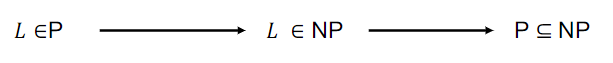
\includegraphics[width=12cm]{pictures/pnp.PNG}
              \item Für viele wichtige Probleme ist jedoch unbekannt, ob sie in P (effizient) lösbar sind
              \item Unbekannt ob $P \neq NP$
              \item Intuitive Frage: Ist das Finden eines Beweises schwieriger als dessen Überprüfung?
              \item[] $\Rightarrow$ Ja, also $P \neq NP$ gilt
              \item In den letzten 50 Jahren kein Beweis für $P = NP$
              \item Eines der wichtigsten offenen Probleme der theoretischen Informatik
              \item Konsequenzen eines Beweises von $P=NP$:
                    \begin{itemize}
                        \item $P=NP$: \fatsf{dramatisch}, vieles bisher schwieriges lösbar (Rucksack, Kryptographie)
                        \item $P\neq NP$: \fatsf{nicht dramatisch}, mgl. interessante Konsequenzen in Kryptographie
                    \end{itemize}
          \end{itemize}
          \clearpage
    \item \fatsf{NP-Vollständigkeit}
          \begin{itemize}
              \item Problem befindet sich in NP
              \item Problem ist so \string"schwer\string" wie jedes Problem in NP
              \item Beweis: Zeigen, dass kein effizienter Algorithmus existiert
              \item Werkzeug: Reduktionen (zum Vergleich verschiedener Probleme)
              \item \textit{NP-Härte/NP-Schwere:}
                    \begin{itemize}
                        \item Klassifikation von Problemen als schwierig, trotz fehlender genauer Zuordnung
                        \item \textit{Starke Indikatoren}, dass Problem $L$ nicht in P ist:
                              \begin{itemize}
                                  \item $L$ ist mindestens so schwierig, wie alle anderen Probleme in NP
                                  \item Daraus folgt, dass $L$ nur in P, wenn $P=NP$ (unwahrscheinlich )
                              \end{itemize}
                    \end{itemize}
              \item \textit{Definitionen}
                    \begin{itemize}
                        \item Problem $L$ ist \fatsf{NP-schwer}, wenn $L' \leq_p L$ für alle $L' \in NP$
                        \item Problem $L$ ist \fatsf{NP-vollständig}, wenn $L$ sowohl NP-schwer als auch in NP ist
                        \item z.B.: Hamilton-Kreis ist NP-vollständig
                    \end{itemize}
          \end{itemize}

          \pagebreak

    \item \fatsf{Reduktionen}\index{Reduktion}
          \begin{itemize}
              \item \textit{Reduktionsidee}
                    \begin{itemize}
                        \item Betrachte Problem $A$, das wir in polynomieller Zeit lösen wollen
                        \item Bereits bekannt: Problem $B$ (in polynomieller Zeit lösbar)
                        \item Benötigt wird Prozedur, die Instanzen der Probleme ineinander überführt
                        \item[] $\Rightarrow$ Transformation benötigt polynomielle Zeit
                        \item[] $\Rightarrow$ Antworten sind gleich
                        \item[] 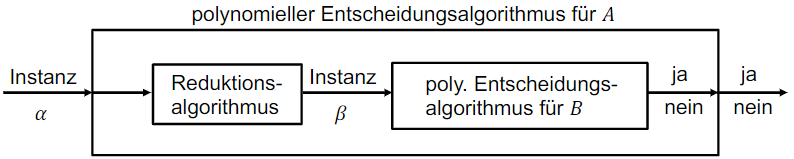
\includegraphics[width=15cm]{pictures/reduktion1.PNG}
                    \end{itemize}

              \item \textit{Beispiel:}
                    \begin{itemize}
                        \item Intuitiv: Reduktion von A auf B, wenn Umformulierung möglich
                        \item[] $\Rightarrow$ Jede Instanz A kann leicht in Instanz von B umformuliert werden
                        \item[] $\Rightarrow$ Lösung der Instanz B liefert Lösung von Instanz A
                        \item Reduktion: Lösen von linearen Gleichungen auf quadratische Gleichnungen
                              \begin{itemize}
                                  \item Lineare Gleichung $ax + b = 0$ $\Rightarrow$ $x= \frac{-b}{a}$
                                  \item Quadratische Gleichung $ax^2 + bx + 0 = 0$ $\Rightarrow$ $x = \frac{-b}{a}, x = 0$
                                  \item Quadratische Gleichung liefert also auch Lösung für lineare Gleichung
                              \end{itemize}
                    \end{itemize}

              \item \textit{Formale Definition:}
                    \begin{itemize}
                        \item[]
                              A lässt sich auf B in \fatsf{polynomieller Zeit reduzieren}, mit Schreibweise $A \leq_p B$, wenn eine
                              in polynomieller Zeit berechenbare Funktion $f: \{0,1\}^* \rightarrow \{0,1\}^*$ existiert, sodass
                              für alle $x \in \{0,1\}^*$ gilt: \\
                              \centerline{$x \in A$ genau dann, wenn $f(x)\in B$}
                        \item[] 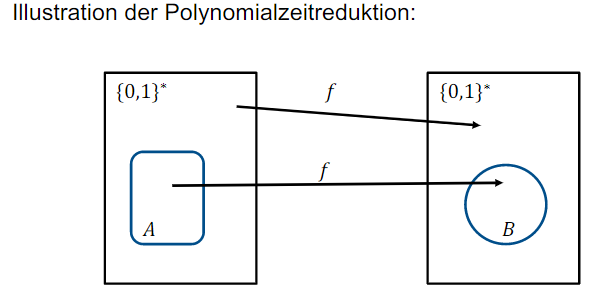
\includegraphics[width=12cm]{pictures/reduktion2.PNG}
                    \end{itemize}
          \end{itemize}

          \pagebreak

    \item \fatsf{Travelling-Salesman Problem}\index{Travelling-Salesman Problem}\\
          
\includegraphics[width=.5\textwidth]{pictures/traveling_salesman.png}
    \begin{itemize}
              \item \textit{Beschreibung}
                    \begin{itemize}
                        \item Reisender plant Rundreise durch mehrere Städte
                        \item Start und Ziel ist eine vorgegebene Stadt
                        \item Jede Stadt nur einmal besucjhen
                        \item Ziel: Minimale Reiselkosten
                        \item[] 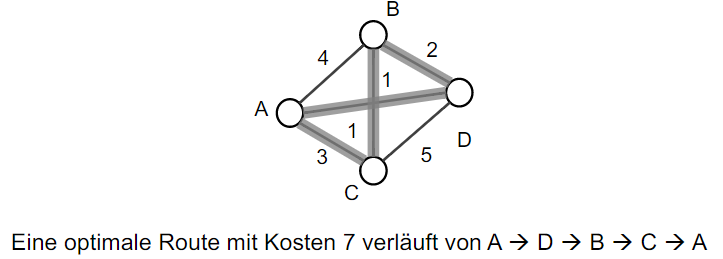
\includegraphics[width=12cm]{pictures/tsp1.PNG}
                    \end{itemize}
              \item \textit{Problem:}
                    \begin{itemize}
                        \item Anzahl der Rundreisen $(n-1)!$
                        \item Stark nach oben explodierende Zahlen
                        \item Brute-Force für große $n$ praktisch unmöglich
                        \item Es existiert kein effizienter Algorithmus, der das TSP effizient löst
                        \item TSP ist \fatsf{NP-vollständig}
                    \end{itemize}
              \item \textit{Beweis NP-Vollständigkeit}
                    \begin{itemize}
                        \item Zeigen: TSP gehört zu NP und TSP ist NP-schwer
                    \end{itemize}
              \item \textit{TSP gehört zu NP}
                    \begin{itemize}
                        \item Gegeben: Instanz des Problems TSP, Folge der $n$ Knoten der Tour (Zertifikat)
                        \item Verifikationsalgorithmus überprüft, ob Folge jeden Knoten genau einmal enthält
                        \item Außerdem Aufsummieren der Kantenkosten und überprüfen, ob diese maximal $k$ ist
                        \item Verifikation läuft in polynomieller Laufzeit $\Rightarrow$ gehört zu NP
                    \end{itemize}
                    \clearpage
              \item \textit{TSP ist NP-schwer}
                    \begin{itemize}
                        \item Wir zeigen $HAM-KREIS \leq_p TSP$
                        \item Start: Instanz von $HAM-KREIS$ mit $G=(V,E)$
                        \item Konstruiere Instanz von $TSP$
                        \item[] $\Rightarrow$ $G'=(V,E')$ mit $E'=\{(i,j):i,j \in V$ und $i\neq j\}$
                        \item Definiere Kostenfunktion $c(i,j) = 0$,falls $(i,j) \in E$ / $c(i,j)=1$, falls $(i,j) \notin E$
                        \item Instanz von TSP ist $<G', c, 0>$ (Konstruktion in polynomieller Zeit) (0: Kosten von 0)
                        \item \fatsf{Zeige jetzt:} $G$ besitzt hamiltonischen Kreis $\Leftrightarrow$ G' enthält Tour mit Kosten $\leq$ 0
                        \item $\Rightarrow$ Graph $G$ besitzt einen hamiltonischen Kreis $h$
                        \item[] 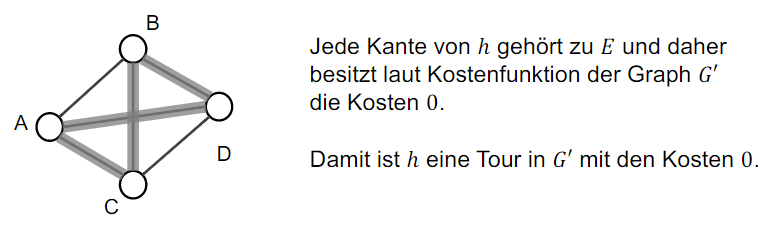
\includegraphics[width=12cm]{pictures/schwer1.PNG}
                        \item $\Leftarrow$ Graph $G$ besitzt eine Tour $h'$ mit Kosten kleiner gleich 0
                        \item[] 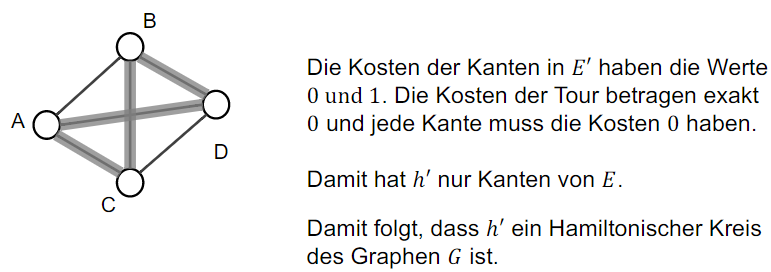
\includegraphics[width=12cm]{pictures/schwer2.PNG}
                    \end{itemize}
          \end{itemize}

\end{itemize}
\end{document}